% main.tex
% Based on AAAS's science_template.tex (v1.1, April 2026) for Science-family journals.
% Single file: main text, then supplement, per that template's structure (not two files).

%%%%%%%%%%%%%%%% START OF PREAMBLE %%%%%%%%%%%%%%%

\documentclass[12pt]{article}

\usepackage{newtxtext,newtxmath}
\usepackage{graphicx}
\usepackage[letterpaper,margin=1in]{geometry}
\linespread{1.5}
\frenchspacing

\renewenvironment{abstract}
	{\quotation}
	{\endquotation}

\date{}

\renewcommand\refname{References and Notes}

\makeatletter
\renewcommand{\fnum@figure}{\textbf{Figure \thefigure}}
\renewcommand{\fnum@table}{\textbf{Table \thetable}}
\makeatother

\usepackage{scicite}
\usepackage{url}

% Per template instructions: do not add further \usepackage{} commands --
% AAAS's conversion software expects a minimal, standard preamble.

%%%%%%%%%%%%%%%% TITLE AND AUTHORS %%%%%%%%%%%%%%%%

% Science Advances limits (Information for Authors, science.org/content/page/
% science-advances-information-authors): title <=135 characters. A "short
% title" (<=50 characters, for the running head) is also required, but is a
% submission-portal metadata field, not manuscript text -- no template macro
% for it, so just a reminder here rather than a fabricated LaTeX command.
% TODO: short title, <=50 characters, for the submission form.
\def\scititle{
	Evidence integration with prediction error\\[0.3em]
	{\large Theory, behavioral experiments, and spiking neural network models}
}
\title{\bfseries \boldmath \scititle}

\author{
	Peter Duggins$^{1\ast}$,
	Alireza Soltani$^{1}$\and
	\small$^{1}$Department of Psychological and Brain Sciences, Dartmouth College, Hanover, NH 03755\and
	\small$^\ast$Corresponding author. Email: psipeter@gmail.com
}

%%%%%%%%%%%%%%%%% END OF PREAMBLE %%%%%%%%%%%%%%%%

\begin{document}

\maketitle

% Science Advances: abstract <=150 words, single paragraph, no citations
% (science.org/content/page/science-advances-information-authors).
\begin{abstract} \bfseries \boldmath
Some abstract text here
\end{abstract}

\section{Introduction}

A really good introduction

\section{Results}

\subsection{Cognitive tasks}
To investigate different aspects of evidence integration and test the generalizability of our model, we studied four evidence-integration tasks (Fig.~\ref{fig:tasks_overview}). Each task presents a sequence of noisy observations and asks for a real-valued estimate after every observation, requiring participants to integrate all evidence observed so far in the trial. The four tasks collectively span multiple dimensions of task design, including input type, sequence length, repetition structure, and estimated quantity. Two of these tasks reanalyze previously published data \cite{prat2024imprecise, yoo2025people}, while two were conducted as part of the current study. Task procedures, stimuli, and participants are detailed in Materials and Methods.

\subsection{Discounted prediction error model}
In the Discounted Prediction Error (DPE) model, the learner maintains a running estimate $V_n$ and, after each observation, computes a prediction error between its current estimate and the new observation, which updates the estimate according to a time-dependent learning rate $\alpha(n)$ (Fig.~\ref{fig:models_overview}A):

\begin{equation}
    \label{eq:dpe_update}
    V_n = V_{n-1} + \alpha(n) \bigl(I_n - V_{n-1}\bigr)
\end{equation}

\noindent The size of this update depends on both a baseline learning rate $\alpha_0$, the number of observations $n$ already accumulated and a discounting parameter $\lambda$:

\begin{equation}
    \label{eq:dpe_alpha}
    \alpha(n) = \frac{\alpha_0}{n^\lambda}
\end{equation}

This single mechanism can reproduce a range of biases documented in the sequential-integration literature. When $\lambda=0$, Eq.~\ref{eq:dpe_alpha} recovers a constant learning rate $\alpha_0$, equivalent to a leaky integrator with fixed update size \cite{usher2001time, glaze2015normative}; when $\lambda=1$, it recovers the unweighted running mean, the statistically optimal estimator under stationary generative statistics. More generally, $\lambda<1$ slows the learning-rate decay and over-weights recent observations (a recency bias), while $\lambda>1$ steepens it and over-weights early observations (a primacy bias); see Supplementary Text for a mathematical proof. Unlike descriptive models that assign each observation its own weight via a post-hoc process (e.g., a weight curve fit directly to the data), DPE generates a range of weighting patterns from a single generative process -- one which runs in real time and does not require a complete memory of past observations. This places DPE within a broader family of models that weight or discount prediction error when updating a running estimate \cite{behrens2007learning, piray2021model, nassar2010approximately, yu2008sequential, camerer1999experience}. These models have been successful in explaining probabilistic reasoning and reward learning across a range of tasks and volatility regimes, but they have not yet been applied to the heterogeneous suite of evidence-integration tasks studied here, used to characterize systematic individual differences in integration strategy, or, most importantly, implemented in a biologically plausible network.

We implemented the DPE model as a spiking neural network (SNN) using the Neural Engineering Framework \cite{eliasmith2003neural}, a method for constructing biologically plausible networks of spiking neurons that realize arbitrary computations (Fig.~\ref{fig:models_overview}B). Three interacting neural populations implement Eqs.~\ref{eq:dpe_update}--\ref{eq:dpe_alpha}, leading to the expected DPE dynamics (Fig.~\ref{fig:models_overview}C): an \textit{error} population computes the prediction error between each observation $I_n$ and the current estimate, discounted by the weight $\alpha(n)$; a \textit{value} population maintains $V_n$ as a working memory through recurrent excitation, updating in response to \textit{error}'s drive and feeding the estimate back for the next comparison; and a \textit{counting} subnetwork tracks the observation index $n$ and decodes $\alpha(n)$ to modulate \textit{error}. Because $\alpha(n)$ emerges from this counting circuit's spiking dynamics, the resulting discounting schedule (and subsequent biases) arises directly from the network's biophysics. Full architectural and simulation details are provided in Materials and Methods.

\subsection{Model performance}
We assessed how well each model accounts for human behavior by fitting its free parameters separately to every participant and computing the root-mean-squared error (RMSE) between each model's predicted responses and the participant's actual responses. We compared DPE and its SNN implementation against three baseline models spanning a range of integration strategies: Mean, which computes the optimal running average with no free parameters \cite{degroot1974reaching}; LeakyIntegrator (LI), which uses the same error-driven update but with a constant learning rate \cite{usher2001time, glaze2015normative}; and PrimacyRecency (PR), which up-weights early and late observations via two independently fit decay parameters \cite{pooley2011understanding, galdo2022quest, yoo2025people}. Model equations and fitting procedures are detailed in Materials and Methods, and were unchanged across tasks; only free parameters were allowed to vary.

DPE achieved the best, or among the best, fit to human behavior on every task (Fig.~\ref{fig:model_performance}). It had significantly lower RMSE than all three baseline models on both Proportion Inference and Value Integration, where it was also the single best-fitting model for the large majority of participants (86\% and 76\%, respectively). On Binary and Continuous Integration, DPE significantly outperformed Mean and LI, but PR matched it on the former and significantly outperformed it on the latter, making PR the modal best-fitting individual model on both (67\% and 70\%, respectively, see Table~\ref{tab:best_fit}). The SNN implementation of DPE remained comparable in RMSE to the baseline models on every task, despite the neural network's spiking representations and constrained connectivity. These RMSE-based rankings were consistent with an independent fit metric, negative log-likelihood (see Supplementary Text).

\subsection{Diminishing response updates}
Overall fit quality, as measured by RMSE, summarizes how closely a model's responses matches human responses on average, but it can obscure whether a model reproduces specific dynamical signatures that characterize how people actually integrate evidence \cite{palminteri2017falsification, wilson2019ten}. For example, a model could achieve a low aggregate error while failing to capture qualitative features of the underlying process, such as perseveration \cite{katahira2018statistical}, confirmation bias \cite{palminteri2017confirmation, palminteri2022computational}, or sequential choice-history effects \cite{yu2008sequential, zhang2014sequential}. We therefore also examined behavioral signatures that reliably emerged in the human data but were not directly targeted by the RMSE fitting procedure, providing a stronger test of whether our model's mechanisms (and not just its output) capture the underlying cognitive processes.

We first investigated the changes that participants made in their responses from observation to observation, specifically whether the magnitude of response change varied as participants integrated more evidence within a trial. For each participant, we computed $|\Delta R|$, the absolute change between one response and the next, and averaged this value across all trials at each point in the sequence (see Materials and Methods); the population-level curve shown in Fig.~\ref{fig:lambda_main}A--C (gray) is the median of these per-participant curves across participants. Response change reliably declined as participants accumulated more evidence within a trial: a per-participant Spearman rank correlation between $|\Delta R|$ and observation number was significantly negative ($p<0.05$) for 85\% of participants in Binary Integration, 59\% in Continuous Integration, and 68\% in Value Integration; Proportion Inference did not show this pattern (see Supplementary Text). DPE, SNN, and PR all reproduced this declining trend (Fig.~\ref{fig:lambda_main}A--C, colors). In contrast, LI's response-change magnitude remained nearly constant across observations due to its fixed learning rate, while Mean always exhibited the same steep decline due to having no free parameters.

The observed decline in response change magnitude resembled the power-law form assumed by DPE. To quantify this pattern, we fit a power-law curve ($A n^{-\lambda}$) directly to each participant's mean $|\Delta R|$ as a function of observation number via nonlinear least squares, and tested whether the fitted discounting rate $\lambda$ was significantly different from zero (see Materials and Methods). The null hypothesis was rejected for 98\% of participants in Binary Integration, 77\% in Continuous Integration, and 72\% in Value Integration. The fitted discounting rate $\lambda$ varied substantially across individuals (Fig.~\ref{fig:lambda_main}D--F). What's more, this individual variation was reliable both within task and (to a lesser extent) across the Binary and Continuous Integration tasks (Fig.~\ref{fig:lambda_sigma_reliability}, see Supplementary Text). Across all three tasks, most participants showed a recency bias ($\lambda<1$), consistent with prior reports in similar sequential-estimation paradigms \cite{yoo2025people, kalm2018visual, baddeley2022recency, feher2017exploration}, but a sizable minority showed either near-optimal integration or a slight primacy bias.

\subsection{Noisy internal representations}
We also examined variability in participants' responses when repeatedly presented with the same evidence sequence. Genuine trial-to-trial variability under exact repetition must reflect noise in mental representations, computations, or responses, but the cognitive and neural mechanism of this noise remains unclear. Prior work analyzed response variability in the Proportion Inference task (whose binary inputs naturally recur across trials) and argued that only models that feature compounding state noise could explain human behavior \cite{prat2024imprecise}. We extended these methods to the Binary and Continuous Integration tasks by ensuring that the initial observations in each trial recurred a minimum number of times across trials, producing partial repetition within each task (see Materials and Methods). We then defined $\sigma$ as the standard deviation of a participant's responses across trials sharing an identical sequence, averaged across all repeated sequences within a task (see Materials and Methods). Response noise $\sigma$ varied substantially across individuals in each task (Fig.~\ref{fig:sigma_main}A--C), and this variation was highly reliable both within task and across the Binary and Continuous Integration tasks, indicating that some individuals consistently represent, update, and/or report their beliefs more precisely than others, regardless of the specific evidence being integrated (Fig.~\ref{fig:lambda_sigma_reliability}, see Supplementary Text).

First, we measured how $\sigma$ grew within a repeated sequence (see Materials and Methods). Human $\sigma$ grew substantially larger as more of the repeated sequence was observed (Fig.~\ref{fig:sigma_main}D--F, gray). This compounding growth in response variability suggests that noise persists within an internal, evolving state representation, rather than arising anew, independently, each time a response is generated. Second, we measured the autocorrelation of participants' residual responses to a repeated sequence, as a function of lag (see Materials and Methods). Human residuals were strongly and positively correlated at short lags, decaying gradually as lag increased (Fig.~\ref{fig:sigma_main}G--I, gray), indicating that this state noise persists across trials but is gradually overwritten as additional, independent noise accumulates.

The models introduced so far produce a single, deterministic response to any given evidence sequence, and therefore cannot immediately account for the response variability just described. A standard solution is to introduce noise at the point of response generation, either by selecting among possible responses probabilistically \cite{sutton2018reinforcement} or by adding independent noise directly to a model's continuous-valued response \cite{nassar2010approximately, piray2021model}. We implemented the latter for each of our mathematical models (Mean, LI, PR, and DPE), adding independent Gaussian noise to each model's predicted response and fitting each participant's own noise magnitude by maximizing the likelihood of their observed responses (negative log-likelihood); this noise term is thus fit to capture that participant's own overall response variance. Out of all the models tested, only SNN reproduced both the growth in $\sigma$ and the decaying positive autocorrelation (Fig.~\ref{fig:sigma_main}D--I, colors). This dissociation confirms that these dynamic behavioral signatures reflect genuine state noise, which naturally arises from spiking activity in SNN's persistent internal representations, but is absent from response-noise-augmented models. These findings are consistent with a noisy-state-based model that explains response variability in the Proportion Inference task \cite{prat2024imprecise}, but SNN grounds this noise in biologically plausible mechanisms and generalizes it across diverse tasks.

\subsection{Neural network predictions}
To further link the neural mechanisms and behavioral phenomenon of evidence integration, and to generate predictions that could validate or falsify our model, we next ran several simulated experiments using SNN in the Continuous Integration task. We began by simulating an outlier paradigm, in which SNN observed a run of three consistent observations followed by one surprising outlier (e.g. 49, 51, 50, 65). Following the outlier, the decoded prediction error (PE) rose sharply before decaying back toward baseline prior to the next observation (Fig.~\ref{fig:neural_main}A). Both the peak PE response and its subsequent decay rate scaled with the network's synaptic learning rate $\alpha_0$ (Fig.~\ref{fig:neural_main}B; peak: $r$=0.91; decay rate: $r$=0.95; both $p$<0.0001). Consequently, the peak PE response strongly predicted the rate at which the PE signal subsequently decayed (Fig.~\ref{fig:neural_main}C; $r$=0.93, $p$<0.0001).

We then asked how the discounting rate $\lambda$ influences SNN's spiking activity alongside its response change decay. We simulated SNN across a range of $\lambda$ values and measured how strongly the spiking activity of error-selective neurons declined across the trial (Fig.~\ref{fig:neural_main}D), quantifying this decline as the percent decrease from early to late observations within a trial. Both this neural activity decay and the network's own behavioral response-change decay became steeper as $\lambda$ increased (Fig.~\ref{fig:neural_main}E; activity decay: $r$=0.89; response-change decay: $r$=0.92; both $p$<0.0001). A decline in neural activity therefore predicted a decline in response change as more evidence was integrated within a trial (Fig.~\ref{fig:neural_main}F; $r$=0.86, $p$<0.0001).

Finally, we tested whether spike noise in SNN is a direct source of behavioral response variability $\sigma$. Qualitatively, SNN's value estimate tracked the ideal target more closely in larger networks than in smaller ones, both within and across trials (Fig.~\ref{fig:neural_main}G). To quantify this relationship while controlling for value drift before the current observation, we simulated another outlier experiment and computed the ``PE noise'', a coefficient-of-variation metric equal to the standard deviation of the decoded PE response (normalized as a percentage of its own mean magnitude) at response time. We also measured the subsequent response variability $\sigma$. We repeated this experiment for multiple network sizes and random sequences, and found that both PE noise and $\sigma$ declined as network size increased (Fig.~\ref{fig:neural_main}H; PE noise: $r$=-0.69; $\sigma$: $r$=-0.88; both $p$<0.0001). PE noise thus directly predicted $\sigma$ across network sizes (Fig.~\ref{fig:neural_main}I; $r$=0.68, $p$<0.0001), confirming that spiking noise in error-selective neurons is a direct source of behavioral response variability.

\subsection{Synaptic versus recurrent implementations}
Having established a neural mechanism that jointly accounts for behavioral and neural signatures of evidence integration, we asked whether these conclusions depend on the specific circuit implementation of DPE, or whether they generalize to a different neural substrate. Our SNN implementation of DPE maintains its running estimate $V_n$ through persistent recurrent activity in the \textit{value} population, consistent with one leading account of how the brain sustains information in working memory \cite{wang2002probabilistic, wang2008decision}. An influential alternative hypothesis, however, proposes that working memory can instead be maintained by synaptic plasticity, without requiring sustained spiking to hold information between observations \cite{mongillo2008synaptic, stokes2015activity}. These two candidate mechanisms can both plausibly implement DPE and are difficult to distinguish from behavior alone. We investigated which neural mechanism is more plausible using a synaptic variant of SNN. This network replaces \textit{value}'s persistent recurrent activity with a synaptic mechanism: a dopamine-like error-driven learning rule instead stores the running estimate $V_n$ in the weights of plastic synapses, updating it only in response to the prediction error signal (Fig.~\ref{fig:synaptic_main}A). These plastic synapses connect a new \textit{etc} population (which fires at a constant, non-selective rate) to \textit{value}, driving it according to a learned transformation (see Materials and Methods).

The synaptic model also captured individual human behavior on the Continuous Integration task, but performed slightly worse than the recurrent model (Fig.~\ref{fig:synaptic_main}B; Wilcoxon $p$<0.0001). To further dissociate the two neural mechanisms, we ran a simulated experiment with a causal perturbation, then compared each model's decoded value trajectory. We injected a band-limited white-noise current, scaled by a strength parameter, into every neuron of the value population during the inter-trial interval (ITI); this perturbation mimics a distractor task or non-invasive brain stimulation delivered during a working-memory delay. Example single-trial dynamics show that both models' decoded estimates are disrupted while the perturbation is active, but only the recurrent model's disruption persists once the ITI ends (Fig.~\ref{fig:synaptic_main}C). Across a range of perturbation strengths, the recurrent model's error (RMSE, relative to the running mean) and response variability ($\sigma$) both grew reliably with perturbation strength (RMSE: $r$=0.77; $\sigma$: $r$=0.58; both $p$<0.0001), while the synaptic model showed no such relationship (both $r\approx0$, $p$>0.9) (Fig.~\ref{fig:synaptic_main}D), confirming that only the recurrent, persistent-activity-based mechanism is vulnerable to a transient disruption of ongoing neural activity.

\section{Discussion}

% TODO -- throughline for this Discussion is NOVELTY, front and center:
% every relationship in Fig.~\ref{fig:neural_main} (rows 1-3) and
% Fig.~\ref{fig:synaptic_main}'s WM-vs-synaptic perturbation dissociation
% is a NOVEL, UNVALIDATED prediction -- no real neural recordings or
% perturbation data exist for this task to check them against. State this
% explicitly, once, covering both figures together (they make the same
% kind of claim -- a testable dissociation/relationship, not yet a
% validated finding), and tie it to Goal 4's framing (docs/SCIENCE.md) of
% testable predictions for future joint neural/behavioral work. This is
% the section's main point, not a caveat to bury at the end.
% Secondary, still worth a sentence: why alpha_0 controls BOTH peak PE
% magnitude and decay rate (Fig.~\ref{fig:neural_main}A-C) is a fact
% about THIS neural implementation, not a direct mathematical consequence
% of the DPE equation itself (Fig.~\ref{fig:models_overview}A) -- don't
% leave it as an unexplained empirical correlation, but keep it
% subordinate to the novelty framing above.
%
% TODO -- per-experiment empirical validation recipes, MOVED OUT of
% Results (Section 2.6 now reports only the simulated findings; per
% instruction, each experiment's own "how this could be tested on real
% data" sentence belongs here instead). Fold these three into the
% novelty paragraph above, one per neural_main row, rather than losing
% them:
%   Row 1 (outlier / alpha_0): test by decoding spikes from error-
%     sensitive neurons during the cue period of an evidence-integration
%     task -- a larger PE response to a surprising observation should
%     also show a faster subsequent decay of that response.
%   Row 2 (activity decay / lambda): test by measuring firing rates of
%     error-sensitive neurons at cue onset and the subsequent response
%     changes after each observation -- individuals whose neural signal
%     declines faster within a trial should also show a faster
%     behavioral decline in response updating.
%   Row 3 (spike noise / n_neurons): test by relating the trial-to-trial
%     reliability of decoded neural signals to an individual's own
%     behavioral response noise sigma.
%   synaptic_main (recurrent vs. synaptic ITI perturbation, Section 2.7):
%     test by applying a distractor task or non-invasive brain stimulation
%     during a working-memory delay in a real evidence-integration
%     experiment and asking whether decoding accuracy recovers once the
%     delay ends (consistent with a recurrent, persistent-activity
%     mechanism) or persists disrupted/unaffected throughout (consistent
%     with a synaptic mechanism).
%
% TODO -- restore a dangling cross-reference: Section 2.6's third
% paragraph (spike noise / n_neurons, Fig.~\ref{fig:neural_main}G-I) used
% to point readers to a second, decoder-free reliability metric
% (split-half spike-count r, corroborating the PE-noise-vs-sigma finding
% from an independent angle) in the Supplementary Text's "A decoder-free
% corroboration of the neurons-vs-SNR result" section -- that pointer was
% lost in a later edit and Results currently has NO reference to that SI
% section at all. Do NOT just re-add the \ref yet: that SI section is
% still its own STUB (the supplementary figure it describes has not been
% built -- see its own TODO there, and docs/SCIENCE.md's "Future
% extensions"). Once that figure exists, add back a parenthetical to
% Section 2.6's third paragraph (e.g. "(see Supplementary Text for a
% second, decoder-free reliability metric that corroborates this
% relationship)") -- tracked here so it isn't lost twice.
%
% TODO -- revisit DPE's relationship to previous weighted-prediction-error
% models here (see Results' DPE subsection, which only disambiguates DPE
% from surprise-modulated adaptive-learning-rate models in 1-2 sentences
% and defers the real argument to here). Now that lambda/sigma results
% are in hand: does a fixed power-law discount schedule suffice to
% explain the observed individual differences and decay patterns, or does
% the data actually call for a surprise/volatility-modulated rate the way
% Behrens/Nassar/Yu-Dayan-style models assume? Make the argument with the
% actual results, not just in the abstract.
% FORMAL STATEMENT (drafted for M&M's "Computational models" subsection,
% then pulled per instruction -- not interpretive, so it belongs here
% instead, as raw material for the argument above rather than a
% restatement of it): DPE belongs to a broader family of models that
% update a running estimate via a weighted prediction error, V_n =
% V_{n-1} + alpha_n(I_n - V_{n-1}) (behrens2007learning, piray2021model,
% nassar2010approximately, yu2008sequential, camerer1999experience).
% These share DPE's basic update form but differ in how alpha_n itself
% is computed: adaptive-learning-rate models estimate alpha_n online as
% a function of observed surprise or an evolving volatility estimate, so
% it can rise or fall from one observation to the next; DPE instead
% fixes alpha_n = alpha_0/n^lambda (Eq.~\ref{eq:dpe_alpha}) as a
% deterministic function of the observation count n alone, via two
% parameters fit once per participant and held constant across a trial,
% rather than an online, surprise-dependent rule with its own separate
% parameters and dynamics. That contrast is exactly the raw material for
% this TODO's own question (does a fixed schedule suffice, or does the
% data call for a volatility-modulated rate) -- state the mechanism
% difference plainly before making the argument.
%
% TODO -- EWA comparison (from prior reviewer correspondence, Reviewer #2):
% EWA (Camerer & Ho 1999, \cite{camerer1999experience}) uses two independent
% mechanisms -- experience weight rho (N(t) = rho*N(t-1) + 1, governing
% accumulation/decay of past observations) and attraction decay phi
% (A(t) ~ phi*A(t-1)) -- that together primarily produce a RECENCY effect;
% primacy only emerges in the limiting case rho=1, phi=1 (no decay at all).
% DPE, by contrast, produces a full primacy-to-recency continuum from a
% single parameter (lambda) at every value, not just a limiting case --
% DPE is NOT a special case of EWA, and exhibits richer primacy effects.
% Also worth keeping from the reviewer response: EWA has mainly been
% applied to economic/multi-agent games with counterfactual reasoning and
% complex inter-choice dependencies, rarely to non-social RL tasks, and
% (as far as we know) never to the sequential-estimation tasks studied
% here -- genuine novelty, not just a reimplementation of an established
% approach.
Lots of discussion
\subsection{Limitations}
Science Advances explicitly requires a limitations paragraph in Discussion

\section{Materials and Methods}

\subsection{Cognitive tasks}

\subsubsection*{Proportion Inference task}
Participants ($n=21$) viewed a box containing red and green rings and, after each of 5 sequentially-revealed rings, moved a slider (0\% to 100\% red) to report their current estimate of the proportion of red rings in the box \cite{prat2024imprecise}. Each participant completed 200 such trials. Because each trial's binary sequence was drawn independently from only $2^5=32$ possible sequences, many trials recurred exactly for a given participant, allowing responses to the same preceding sequence to be compared across repeated presentations. Note that, unlike the other tasks, this task asks participants to estimate something about an unknown distribution (the proportion of balls in the box), rather than summarize the sequence up to the current observation.

\subsubsection*{Binary Integration task}
Participants ($n=46$) viewed a sequence of red and blue balls, presented one at a time, and moved a slider after each observation to report their running estimate of the proportion of blue balls observed so far. Each of 32 trials consisted of 15 observations drawn from an independently-sampled target proportion. As in the Proportion Inference task, a subset of trials coincidentally shared identical initial observations by chance, allowing for a repeated-sequence comparison up to the fifth observation.

\subsubsection*{Continuous Integration task}
Participants ($n=46$) viewed a sequence of numbers, presented one at a time and each drawn from a hidden normal distribution (mean ranging from 15 to 85, fixed standard deviation of 10), and moved a slider after each observation to report their running estimate of the sequence's average. Each of 32 trials consisted of 15 observations. To ensure the repetition of sequences required to calculate $\sigma$, the first 4 observations of every trial were deliberately drawn from a shared pool of 8 fixed sequences, each repeated across 4 trials, producing designed rather than coincidental repetition at the beginning of each sequence.

\subsubsection*{Value Integration task}
Participants ($n=38$) viewed pairs of snack images, presented sequentially on opposite sides of the screen, and moved a joystick-controlled slider to report their running estimate of the average value difference between the left and right snacks \cite{yoo2025people}. Snacks were rated for individual desirability by each participant beforehand. Each of 15 trials included 30 such image pairs; sequences were never repeated within or across participants.

\subsection{Participants}
Participants for the Binary and Continuous Integration tasks were recruited through Prolific, restricted to an approval rating of at least 90\%, more than 20 previously completed studies, and fluent English. 79 and 78 participants completed the Binary and Continuous Integration tasks, respectively (a small number of additional sessions were terminated early due to repeated response timeouts, or were left incomplete); after applying the exclusion criterion described below, and requiring a valid session in both tasks, 46 participants were retained, drawn from the same pool of individuals in both tasks. All participants provided informed consent electronically, reading a series of disclosures and checking a box affirming they had read and agreed to participate before beginning, under a protocol approved by the Committee for the Protection of Human Subjects at Dartmouth College. Participants were compensated \$5 for completing each task, plus up to an additional \$5 based on task performance, with a median completion time of approximately 41 minutes per task, corresponding to an effective hourly wage of approximately \$7--15 depending on performance.

We excluded participants whose responses did not reliably depend on observations prior to the most recent one within a trial (``non-integrators''), since such responses provide no sign of evidence integration, regardless of the integration strategy used or the accuracy of their final responses. This single test catches participants who exhibit a variety of disengaged response patterns (such as simply reporting whatever observation they just saw), without penalizing participants who integrate evidence inaccurately or with unusual weighting. For each participant and task, we regressed each response on the current observation's value and the expanding mean of all strictly prior observations within that trial, fit per trial and aggregated across trials. We constructed a 95\% confidence interval on the prior-observations coefficient via a trial-level cluster bootstrap (resampling trials with replacement, 20,000 resamples), and retained a participant only if this interval excluded zero. Participants with fewer than 8 trials, or fewer than 10 total observations, in a task were excluded outright as too little data to test reliably. This criterion was applied per task, but a participant excluded in either task was excluded from both, so the same 46 participants are analyzed in both Binary and Continuous Integration.

\subsection{Computational models}
We compared DPE (Eqs.~\ref{eq:dpe_update}--\ref{eq:dpe_alpha}) against three baseline models.

\subsubsection*{Mean}
Mean computes the unweighted running average of all observations so far:
\begin{equation}
    V_n = \frac{1}{n}\sum_{i=1}^n I_i
\end{equation}
Mean has no free parameters, and its output is implicitly bounded to the valid response range $[-1,1]$ by construction.

\subsubsection*{LeakyIntegrator (LI)}
LI applies the same error-driven update as DPE, but with a constant learning rate $\alpha_{LI}$ rather than one that decays with $n$:
\begin{equation}
    V_n = V_{n-1} + \alpha_{LI}\left(I_n - V_{n-1}\right)
\end{equation}
LI's single free parameter is $\gamma \in [0,1]$, with $\alpha_{LI} = 1-\gamma$; LI's update was clipped to $[-1,1]$ after each observation. LI is thus equivalent to DPE with $\lambda=0$ and $\alpha_0 = 1-\gamma$: a constant, non-decaying learning rate.

\subsubsection*{PrimacyRecency (PR)}
PR computes a weighted average of all observations using a temporal weighting function \cite{pooley2011understanding, galdo2022quest}:
\begin{equation}
    V_n = \frac{\sum_{o=1}^n w(o,n)\, I_o}{\sum_{o=1}^n w(o,n)}
\end{equation}
\begin{equation}
    w(o,n) = \left[1 - \left(1-\varepsilon_p^{o}\right)\left(1-\varepsilon_r^{\,n-o+1}\right)\right](1-\eta) + \eta
\end{equation}
PR's two free parameters, $\varepsilon_p, \varepsilon_r \in [0,1]$, control primacy and recency weighting respectively; $\eta=0.01$ is fixed \cite{yoo2025people}. PR's output is implicitly bounded to $[-1,1]$ by construction.

\subsubsection*{Proportion Inference response transform}
On the Proportion Inference task, every model's raw estimate $V_n$ was additionally rescaled before comparison to human responses:
\begin{equation}
    \label{eq:laplace}
    V_n \to V_n \cdot \frac{n}{n+2}
\end{equation}
a Laplace-smoothing correction equivalent to the optimal Bayesian estimate of a probability under a uniform prior (adding one pseudo-observation of each outcome before dividing), reflecting this task's distinct estimand (see Cognitive Tasks).

\subsection{Neural network model}

\subsubsection*{Neural Engineering Framework}
In the Neural Engineering Framework (NEF), spiking activity within a population of neurons represents cognitive states such as value estimates, prediction errors, or weights. These states are defined as vectors that change with the network's spiking activity, and we can decode these vectors from the underlying spiking activity, or encode new vectors into spiking activity by driving neurons with an external current. Together, encoding and decoding define the concept of representation in an NEF network, and the framework provides equations that quantify how these processes occur biologically. A key aspect of representation in the NEF is population coding: each neuron in a population is sensitive to the represented state to a different degree, specified by that neuron's own random tuning curve, so only by decoding from many neurons together can a reliable estimate of the represented quantity be recovered.

Functionally, the NEF can implement any linear or non-linear dynamical system in a network of spiking neurons, effectively compiling a mathematical description of a cognitive computation (here, Eqs.~\ref{eq:dpe_update}--\ref{eq:dpe_alpha}) into a network that implements it. To transform represented states into new states, the NEF specifies synaptic connection weights between (or within) populations. For example, \textit{error} receives one connection carrying the current observation $I_n$ and another carrying \textit{value}'s own estimate with a negative transform, so that \textit{error} comes to represent their difference, $I_n - V_{n-1}$. Its connection to \textit{value}, in turn, is specified with a nonlinear function that computes the product of \textit{error}'s two represented dimensions, $\alpha(n)(I_n-V_{n-1})$, rather than a linear combination of them.

Critically, although the NEF provides tools for representing and transforming cognitive states, it does not dictate a unique network architecture: many configurations of neural populations and synaptic connections can implement the same high-level computation. Specifying a network architecture therefore amounts to a hypothesis about which brain areas represent which cognitive states, and how they are connected to perform the required transformations. This is exactly the hypothesis under comparison between the recurrent and synaptic implementations described below. For a more thorough introduction to the NEF, and examples of the range of cognitive and neural models built using it, see \cite{eliasmith2003neural, eliasmith2013build, choo2018spaun, dumont2023biologically, duggins2022constructing, duggins2023learning, rasmussen2017neural, duggins2022reinforcement, bartlett2023improving, duggins2024spiking, duggins2024scalable, dumont2022, stockel2021connecting}.

\subsubsection*{Recurrent implementation}
We implemented DPE (Eqs.~\ref{eq:dpe_update}--\ref{eq:dpe_alpha}) as a spiking neural network (SNN) using the NEF. The network comprises populations of spiking leaky-integrate-and-fire (LIF) neurons connected via current-based synapses, two mechanisms widely regarded as a compromise between biological realism and computational efficiency \cite{eliasmith2013build, duggins2022constructing, gerstner2014neuronal, dayan2005theoretical}. In its default (recurrent) configuration, the network comprises three main populations (Fig.~\ref{fig:models_overview}B): \textit{error}, \textit{value}, and a counting network, \textit{count} (described below). \textit{Error} is two-dimensional, representing the discounting weight $\alpha(n)$ (received from \textit{count}) and the raw prediction error $I_n - V_{n-1}$ (received from the current observation and feedback from \textit{value}). A single connection from \textit{error} to \textit{value} computes the product of these two represented dimensions, $\alpha(n)(I_n-V_{n-1})$ (the weighted prediction error of Eq.~\ref{eq:dpe_update}), and adds it into \textit{value}'s own input. \textit{Value} is one-dimensional and represents the running estimate $V_n$. In this recurrent implementation, \textit{value} maintains $V_n$ via a recurrent connection (synaptic time constant $\tau_{fb}=0.2$s), so that $V_n$ persists as ongoing recurrent activity between observations.

Each observation was presented as an input pulse for $t_{obs}=1.5$s, followed by an inter-trial interval (ITI) of $t_{iti}=0.5$s. During the ITI, the input was silenced, and \textit{error} was inhibited in one of two ways to prevent \textit{value} from converging toward a nonsensical $I_n=0$. By default, \textit{error}'s own neurons were inhibited directly, fully blocking its activity until the next observation. For the recurrent-vs-synaptic perturbation experiment (see Simulated neural network experiments), we instead inhibited an intermediate \textit{gate} population carrying \textit{value}'s feedback to \textit{error}, allowing \textit{error} to continue driving learning throughout the ITI, which was necessary for injected noise to have any effect during that window. We verified that the choice of inhibition mechanism made little difference to the network's overall dynamics. Model responses were decoded from \textit{value}'s spiking activity 0.5s into each observation period. By default, \textit{error} and \textit{value} each contain 500 neurons and \textit{count} contains 2500 neurons.

\subsubsection*{Synaptic implementation}
An alternative implementation replaces \textit{value}'s persistent recurrent activity with a synaptic mechanism (Fig.~\ref{fig:synaptic_main}A). Rather than a recurrent connection, \textit{value} instead receives input from a new population, \textit{etc}, which fires at a constant, non-selective rate; its own activity carries no information about $I_n$ or $V_n$. As in the recurrent implementation, \textit{error}'s access to \textit{value}'s feedback was silenced during the ITI (see above). \textit{Etc} comprised 500 neurons, the same as \textit{error} and \textit{value}. The connection from \textit{etc} to \textit{value} is plastic, initialized to zero and updated online via the Prescribed Error Sensitivity (PES) rule \cite{macneil2011fine}, a biologically motivated, spike-based error-driven learning rule capable of learning weights that compute a wide range of functions \cite{voelker2015solution}:
\begin{equation}
    \label{eq:pes}
    \Delta\omega_{ij} = \kappa\, a_i\, (\epsilon_j \cdot E_n)
\end{equation}
where $\omega_{ij}$ is the weight between presynaptic neuron $i$ (in \textit{etc}) and postsynaptic neuron $j$ (in \textit{value}), $\kappa=4\times10^{-4}$ is a fixed learning rate, $a_i$ is the activity of presynaptic neuron $i$, $\epsilon_j$ is the encoder for postsynaptic neuron $j$, and $E_n$ is the same weighted prediction error $\alpha(n)(I_n-V_{n-1})$ decoded from \textit{error}. Because \textit{etc}'s own spiking pattern carries no information, the entire estimate $V_n$ is encoded in the synaptic weights $\omega_{ij}$ themselves, rather than in any ongoing spiking activity: an ``activity-silent'' storage mechanism \cite{mongillo2008synaptic, stokes2015activity}.

\subsubsection*{Counting network}
Both the recurrent and synaptic implementations rely on the same counting network, \textit{count}, to track the observation index $n$ and decode the discounting weight $\alpha(n)$ (Eq.~\ref{eq:dpe_alpha}) that modulates \textit{error}. To detect the onset of each new observation, \textit{count} performs approximate differentiation on the raw input stream: an \textit{onset detector} population receives the input through two parallel connections, one with a fast synaptic time constant ($\tau_{fast}=0.01$s) and a positive sign, and one with a slow time constant ($\tau_{slow}=0.2$s) and a negative sign. Because \textit{onset detector}'s neurons are tuned to fire only for positive input, the population emits a brief pulse only on a rising edge of the input, i.e., when a new observation begins, not during the sustained presentation of an observation or during the ITI. These pulses drive a \textit{memory} population, which integrates them over time via a recurrent connection (synapse $\tau_{fb}=0.2$s), accumulating a running count of the observations presented so far. Two linear readouts decode the observation count $n$ and the discounting weight $\alpha(n)=\alpha_0/n^\lambda$ directly from that activity; the latter is what feeds into \textit{error}, as described above. Because $\alpha(n)$ is computed from \textit{memory}'s own imprecise, noisy spiking activity rather than imposed externally, the resulting discounting schedule, and the behavioral and neural signatures that follow from it, emerges directly from the network's own biophysics. In the network's production configuration, \textit{onset detector} contains 500 neurons and \textit{memory} contains 2000 neurons. Note that we rescale \textit{memory}'s representational radius to the maximum observation count for a given task to ensure accurate counting.

\subsection{Parameter fitting}
For each participant and task, we fit each model's free parameters using the tree-structured Parzen estimator sampler implemented in Optuna \cite{optuna_2019}. The loss was the root-mean-squared error (RMSE) between each model's predicted and the participant's own response. To compute it, each participant's own trials were randomly partitioned into $k=5$ disjoint folds, RMSE was computed separately within each fold, and these five values were averaged, producing an in-sample loss metric. We did not attempt genuine nested cross-validation due to the small number of trials per participant: a single held-out fold would be too small to reliably estimate RMSE.

To validate model rankings with an independent fit metric, and to fit each math model's own trial-to-trial response variability, we additionally fit noise-augmented variants of Mean, LI, PR, and DPE via negative log-likelihood (NLL). Each variant's deterministic response was computed once per Optuna trial, then an ensemble of 100 simulated responses was generated by adding independent Gaussian noise, $\mathcal{N}(0,\sigma_{resp}^2)$, to that response and clipping to $[-1,1]$; $\sigma_{resp}$ was fit as an additional free parameter. The loss was the Gaussian negative log-likelihood of the participant's own observed response under the resulting per-observation ensemble mean and standard deviation (floored at $10^{-3}$ to keep the loss finite):
\begin{equation}
\label{eq:nll}
\text{NLL} = \frac{1}{T}\sum_{t=1}^T \left[\log\hat\sigma_t + \frac{(y_t - \hat\mu_t)^2}{2\hat\sigma_t^2}\right]
\end{equation}
where $y_t$ is the participant's own response at observation $t$, and $\hat\mu_t$, $\hat\sigma_t$ are the ensemble mean and (floored) standard deviation at that same observation. As with RMSE, this loss was averaged across the same 5 folds.

Pairwise comparisons of RMSE distributions across models (Fig.~\ref{fig:model_performance}; Table~\ref{tab:best_fit}) used two complementary approaches. First, for each task, we compared DPE's per-participant RMSE against each baseline model's own RMSE using a paired Wilcoxon signed-rank test (two-sided, $\alpha=0.05$). Second, for each task, we counted the number of participants for whom each model achieved the single lowest RMSE, restricted to participants with a valid fit for every model being compared.

\subsection{Discounting rate ($\lambda$)}
For each participant, we computed $|\Delta R|$, the absolute difference between consecutive responses within a trial, and averaged this value across all trials at each observation, yielding one mean $|\Delta R|$ curve per participant per task (Fig.~\ref{fig:lambda_main}A--C). Proportion Inference was excluded from this and all following analyses in this section, since its response-change curve does not decline systematically (see Supplementary Text). Participants with fewer than 3 defined points in their own curve were excluded from all analyses below.

To test whether $|\Delta R|$ reliably declined within a trial, we computed the Spearman rank correlation between observation number $n$ and each participant's own $|\Delta R|$ curve; a decline was flagged when this correlation was negative with $p<0.05$. To quantify the shape of this decline, we fit a power law, $A n^{-\lambda}$, to each participant's own curve via bounded nonlinear least squares (initial guess $A=0.1$, $\lambda=0.5$; bounds $A,\lambda \in [0,2]$). To test whether the resulting discounting rate $\lambda$ was significantly different from zero, we used the standard error of $\lambda$ from the fit's own covariance matrix in a two-sided $t$-test, with degrees of freedom equal to the number of points in that participant's curve minus 2. Participants whose fit landed within $10^{-3}$ of a parameter bound were excluded from this test, since the covariance estimate is unreliable at a constrained optimum.

We assessed $\lambda$'s reliability in two ways. Within task, we split each participant's own trials into odd and even subsets (interleaved by trial index, not chronological order, to isolate estimation noise from systematic drift or learning over the course of the session). We then refit $\lambda$ separately within each half and computed the Pearson correlation between the two resulting $\lambda$ estimates across participants. Across task, we compared each participant's own $\lambda$ fit on the Binary and Continuous Integration tasks directly (Pearson correlation).

\subsection{Response variability ($\sigma$)}
To measure response variability under exact repetition, we first identified groups of trials, within a participant and task, that shared an identical sequence of initial observations (a ``repeated sequence''). For each repeated sequence, and separately at each shared observation within that sequence, we computed the standard deviation of the participant's responses across trials. Averaging this standard deviation across every observation and every repeated sequence yielded one $\sigma$ value per participant per task (Fig.~\ref{fig:sigma_main}A--C). We only analyzed sequences that repeated at least 3 times, and only measured up to a maximum of 5 observations within a sequence.

To ensure repeated sequences for computing $\sigma$, the Continuous Integration task drew each trial's first 4 observations from one of 8 fixed prefixes, evenly centered across the task's mean range and each repeated across 4 of the 32 trials. Each trial was additionally assigned one of 32 target means, also evenly spread across the same range; trials' prefixes and target means were paired using the Hungarian algorithm, globally minimizing the total mismatch between a prefix's own mean and its assigned target across all 32 trials jointly. Given a trial's prefix and target mean, the remaining 11 observations were drawn so that the full 15-observation sequence's sample mean landed on the target mean in expectation, with an analytic correction to the suffix's own variance so the pooled sequence's expected standard deviation matched the task's fixed value despite the prefix being an independent block. If the achieved standard deviation fell outside tolerance, the suffix was redrawn (up to 100 attempts), and if that still failed for every repeat of a given prefix, the prefix itself was regenerated from scratch.

To measure how $\sigma$ grows within a repeated sequence (Fig.~\ref{fig:sigma_main}D--F), we computed the same standard deviation as above, but separately at each observation rather than averaged across observations, and then averaged across participants at each observation. Each resulting curve was normalized by its own value at its first available observation, so that every curve starts at 1 and growth is expressed relative to each source's own baseline.

To measure the autocorrelation of residual response variability (Fig.~\ref{fig:sigma_main}G--I), we first computed each response's residual: its deviation from that participant's own mean response to the same sequence at the same observation. For each participant and lag $k$, we paired every residual at observation $t$ with the residual at observation $t+k$ within the same trial (pooling across all valid $t$ and across repeated sequences), and computed their Pearson correlation. We then averaged these per-participant correlations across participants at each lag.

We assessed $\sigma$'s reliability using the same two approaches as $\lambda$: within task, by splitting each participant's own trials into interleaved odd and even subsets and recomputing $\sigma$ separately within each half (Pearson correlation between the two); and across task, by comparing each participant's own $\sigma$ on the Binary and Continuous Integration tasks directly (Pearson correlation).

\clearpage

%%%%%%%%%%%%%%%% MAIN TEXT FIGURES %%%%%%%%%%%%%%%
% Per template: figures/tables go at the end of the main text, not inline.
% Science Advances: <=10 figures and tables COMBINED in the main text; each
% caption <=200 words (science.org/content/page/science-advances-information-authors).

\begin{figure}
	\centering
	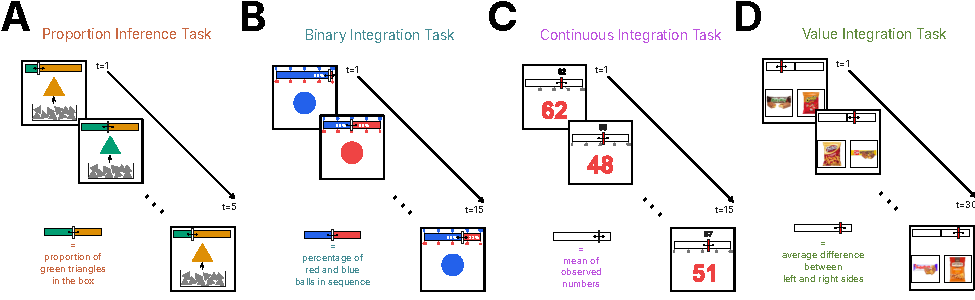
\includegraphics[width=1.0\textwidth]{figures/tasks_overview_paper.pdf}
	\caption{\textbf{Evidence integration in four sequential estimation tasks.} In each task, participants make sequential observations and report a real-valued estimate after each one. Tasks differ in input type, sequence length, and repetition structure. (\textbf{A}) The \textit{Proportion Inference Task} \cite{prat2024imprecise} presents rings of two colors drawn randomly from a box and asks participants to report the hidden proportion of one color. Each trial includes 5 observations, leading to frequent repetition of color sequences. (\textbf{B, C}) The \textit{Binary} and \textit{Continuous Integration Tasks} present binary (continuous) draws from a hidden distribution and ask participants to report a running estimate of the proportion (mean) of the sequence so far. Each trial includes 15 observations, and the first few are drawn from a small pool of fixed sequences, producing partial repetition across trials. (\textbf{D}) The \textit{Value Integration Task} \cite{yoo2025people} presents pairs of snack items and asks participants to report the mean value difference between the accumulated snacks on the left vs right. Each trial includes 30 observations, and snack sequences are never repeated. }
	\label{fig:tasks_overview}
\end{figure}

\begin{figure}
	\centering
	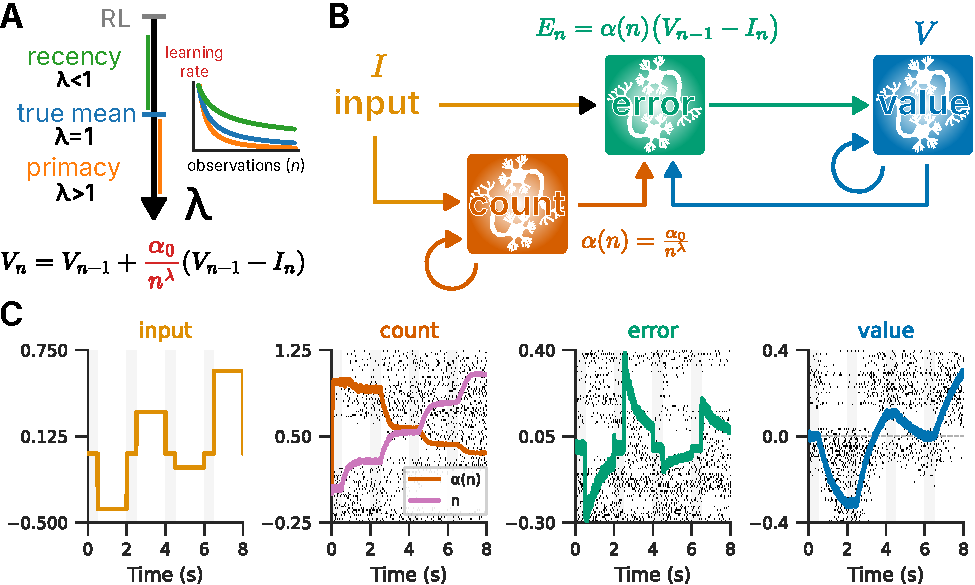
\includegraphics[width=1.0\textwidth]{figures/models_overview_paper.pdf}
	\caption{\textbf{The Discounted Prediction Error (DPE) model and its spiking neural network implementation.} (\textbf{A}) Using an error-driven update rule, the DPE model integrates each observation $I_n$ into its running estimate $V_n$ using a learning rate that decays as a power law of the observation count $n$. The discounting exponent $\lambda$ sets the resulting integration strategy (see Supplementary Text): $\lambda=1$ recovers the unweighted running mean, $\lambda<1$ slows the decay and over-weights recent observations (recency), and $\lambda>1$ steepens it and over-weights early observations (primacy). (\textbf{B}) A spiking neural network implements the same computation using multiple anatomically- and functionally-distinct neural populations. Each observation $I_n$ feeds into \textit{error}, which computes the (discounted) prediction error between the observation and the current value estimate. \textit{Error} then drives \textit{value}, which maintains a working memory of $V_n$ through recurrent excitation and feeds it back to \textit{error} for the next comparison. \textit{Count} tracks the observation number in working memory and decodes the discounting weight $\alpha(n)$ that modulates \textit{error}. (\textbf{C}) Spiking activity (rasters) and decoded traces from one example trial (four observations, shaded inter-trial intervals).}
	\label{fig:models_overview}
\end{figure}

\begin{figure}
	\centering
	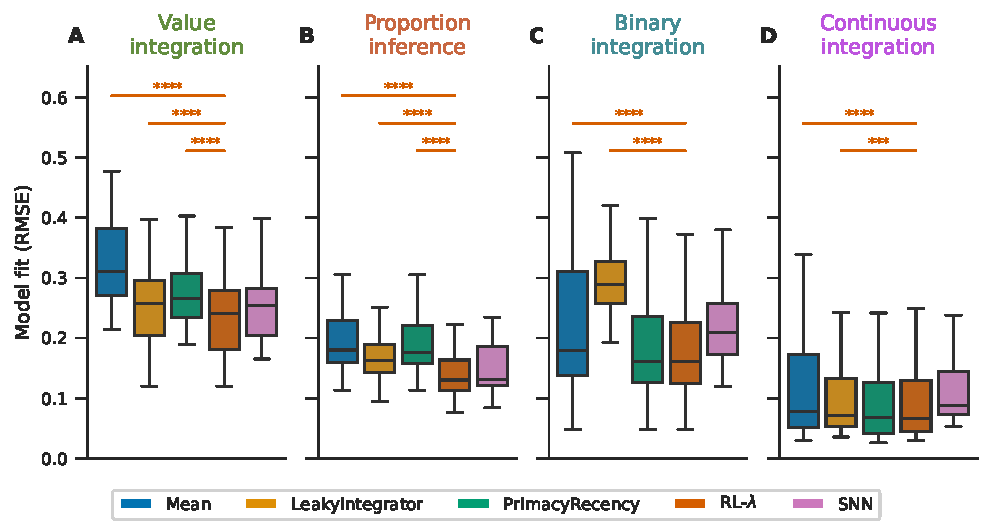
\includegraphics[width=1.0\textwidth]{figures/model_performance.pdf}
	\caption{\textbf{DPE outperforms other integration models on most tasks and the SNN implementation remains competitive despite spiking noise.} Each model was fit separately to every participant via RMSE between predicted and human responses; boxplots show the resulting distribution across participants. Mean computes the unweighted running average \cite{degroot1974reaching}; LI uses prediction error to update its running estimate, but with a constant learning rate \cite{usher2001time, glaze2015normative}; PR up-weighs earlier and more recent observations via two free decay parameters \cite{pooley2011understanding, galdo2022quest}. DPE has significantly lower RMSE than all three baselines on the Proportion Inference (\textbf{A}) and Value Integration (\textbf{D}) tasks (stars: paired Wilcoxon vs.\ DPE), and than Mean and LI on Binary (\textbf{B}) and Continuous (\textbf{C}) Integration; PR ties DPE on Binary Integration and significantly outperforms it on Continuous Integration. SNN, which reproduces DPE's computation within a biologically plausible network, necessarily has higher RMSE than DPE due to spike noise and real-time dynamics, but remains comparable to the other models. Model comparisons were consistent when validated using a second fit metric, negative log-likelihood (see Supplementary Text).}
	\label{fig:model_performance}
\end{figure}

\begin{table}
	\centering
	\caption{\textbf{Best-fitting model (lowest RMSE) per participant, by task.} For each task, the number (and percentage) of participants for whom each model achieved the lowest RMSE, restricted to participants with a valid fit for every model in that task (see Materials and Methods). Bold indicates the model with the most wins in each task.}
	\label{tab:best_fit}
	\begin{tabular}{lccccc}
		\hline
		Task ($n$) & Mean & LI & PR & DPE & SNN \\
		\hline
		Proportion Inference (21) & 0 (0\%) & 2 (10\%) & 0 (0\%) & \textbf{18 (86\%)} & 1 (5\%) \\
		Binary Integration (46) & 0 (0\%) & 0 (0\%) & \textbf{31 (67\%)} & 15 (33\%) & 0 (0\%) \\
		Continuous Integration (46) & 0 (0\%) & 3 (7\%) & \textbf{32 (70\%)} & 9 (20\%) & 2 (4\%) \\
		Value Integration (37) & 0 (0\%) & 7 (19\%) & 0 (0\%) & \textbf{28 (76\%)} & 2 (5\%) \\
		\hline
	\end{tabular}
\end{table}

\begin{figure}
	\centering
	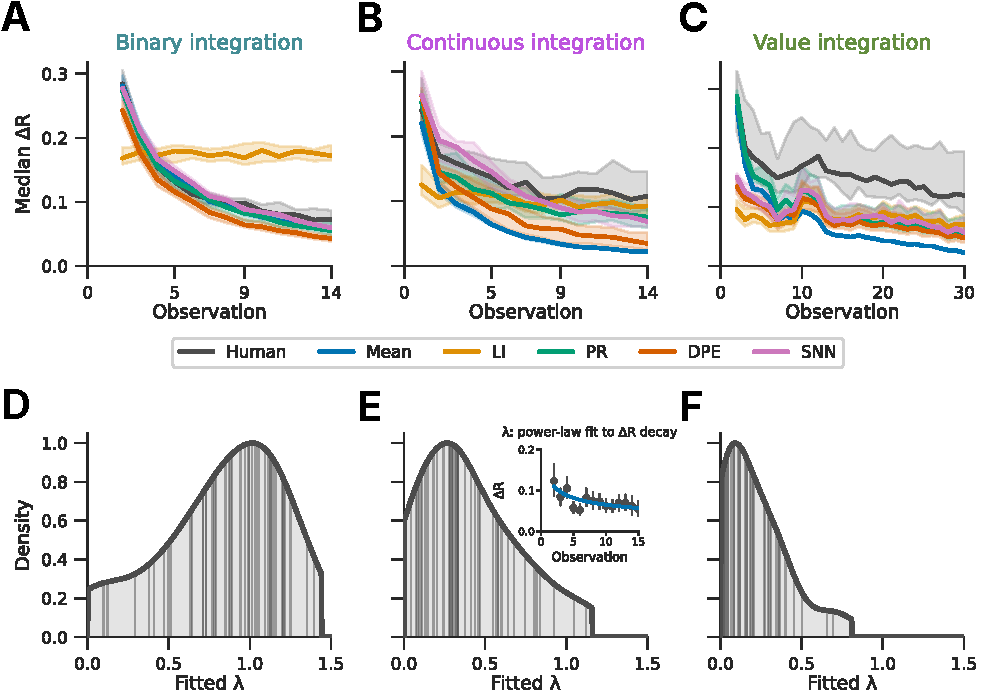
\includegraphics[width=1.0\textwidth]{figures/lambda_main.pdf}
	\caption{\textbf{Magnitude of response change decays with evidence accumulated, and individuals differ systematically in how quickly.} (\textbf{A--C}) Human response change (gray) is the median (across participants) of each participant's $|\Delta R|$ -- the absolute change between one response and the next -- at each point in the sequence, averaged across all sequences, for Binary, Continuous, and Value Integration tasks (Proportion Inference is excluded; see Fig.~\ref{fig:lambda_balls} and Supplementary Text). Response change reliably shrinks as people gather more evidence. (\textbf{D--F}) Fitting a power-law curve to each participant's response-change curve reveals large individual differences in temporal discounting $\lambda$. Consistent with previous work \cite{yoo2025people}, most individuals show a moderate-to-strong recency bias in most tasks ($\lambda<1$), but a substantial minority show near-optimal discounting or even a primacy bias ($\lambda\geq1$). The distribution of $\lambda$ differs across tasks, but individuals show significant consistency in $\lambda$ both within and across tasks (see Supplementary Text). PR, DPE, and SNN all correctly predict this decay, but LI's response-change curve is nearly constant, and Mean cannot capture individual differences.}
	\label{fig:lambda_main}
\end{figure}

\begin{figure}
	\centering
	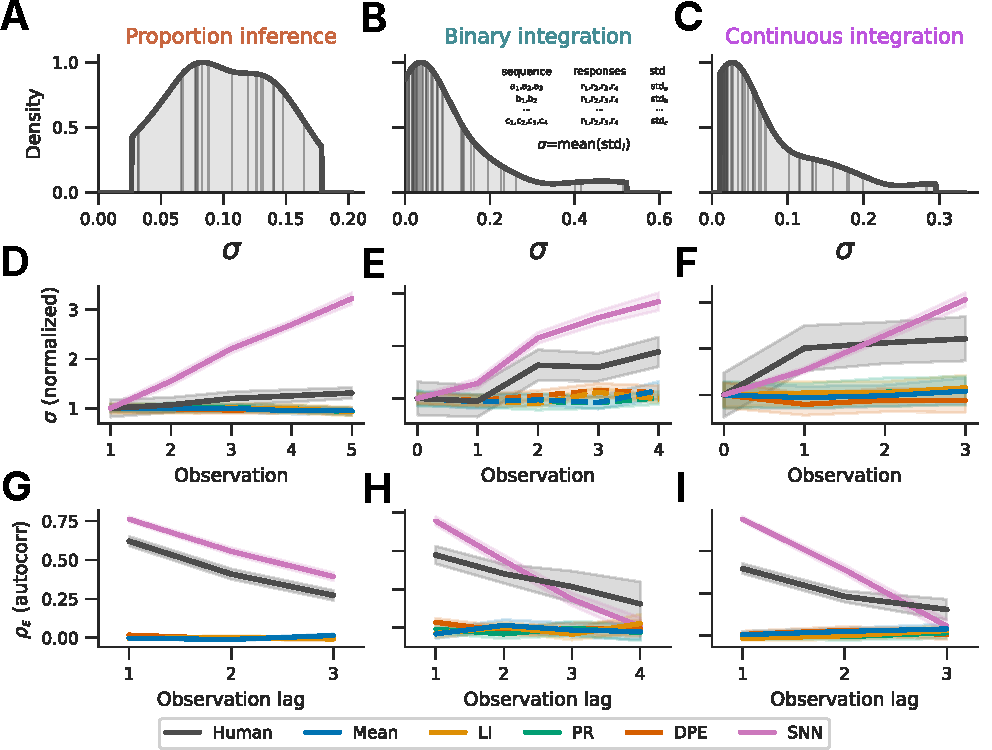
\includegraphics[width=1.0\textwidth]{figures/sigma_main.pdf}
	\caption{\textbf{Only the spiking network reproduces the dynamics of human response variability.} (\textbf{A--C}) Response variability is measured with $\sigma$, the standard deviation of a participant's responses when repeatedly presented with the same short sequence, averaged across all such sequences. $\sigma$ differs systematically across individuals, with significant within- and across-task consistency (Value Integration is excluded because its sequences are never repeated; see Supplementary Text). To investigate the underlying mechanisms, we fit noise-augmented variants of the mathematical models and compared them to SNN and human data. (\textbf{D--F}) Response noise grows over the course of repeated sequences for humans and SNN, but not for the noise-augmented models. (\textbf{G--I}) Trial-wise deviations from a participant's typical response (measureable using repeated sequences) are strongly autocorrelated for subsequent responses in humans and SNN, but not for the noise-augmented models. These two dynamic signatures reflect the ``state noise'' inherent in neural representations, which arise from spike noise and propagate forward in time.}
	\label{fig:sigma_main}
\end{figure}

\begin{figure}
	\centering
	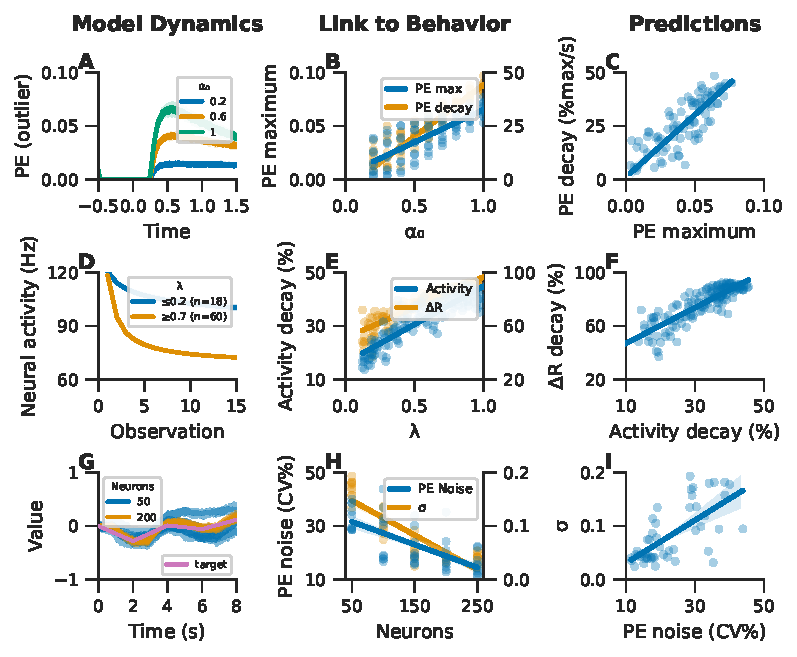
\includegraphics[width=1.0\textwidth]{figures/neural_main.pdf}
	\caption{\textbf{SNN dynamics link neural activity to behavior, yielding novel testable predictions.} Columns show network dynamics for representative parameter values, how neural and behavioral measures of those dynamics scale with key model parameters, and how these measures covary directly, respectively. (\textbf{A--C}) After a run of three consistent observations, one outlier evokes a sharp rise in decoded prediction error (PE) that decays before the next observation; both the peak response and the PE decay rate scale with the synaptic learning rate $\alpha_0$, and the peak PE response directly predicts the subsequent rate of PE decay. (\textbf{D--F}) The activity of error-sensitive neurons decays as evidence accumulates, at a rate set by the synaptic discounting parameter $\lambda$; this neural decay rate directly predicts the behavioral decline in response-change magnitude. (\textbf{G--I}) Spiking noise causes the decoded value estimate to drift across repeated presentations of an identical sequence, at a rate that decreases with the number of neurons engaged; PE noise within trials (normalized coefficient of variation) directly predicts behavioral response variability $\sigma$.}
	\label{fig:neural_main}
\end{figure}

\begin{figure}
	\centering
	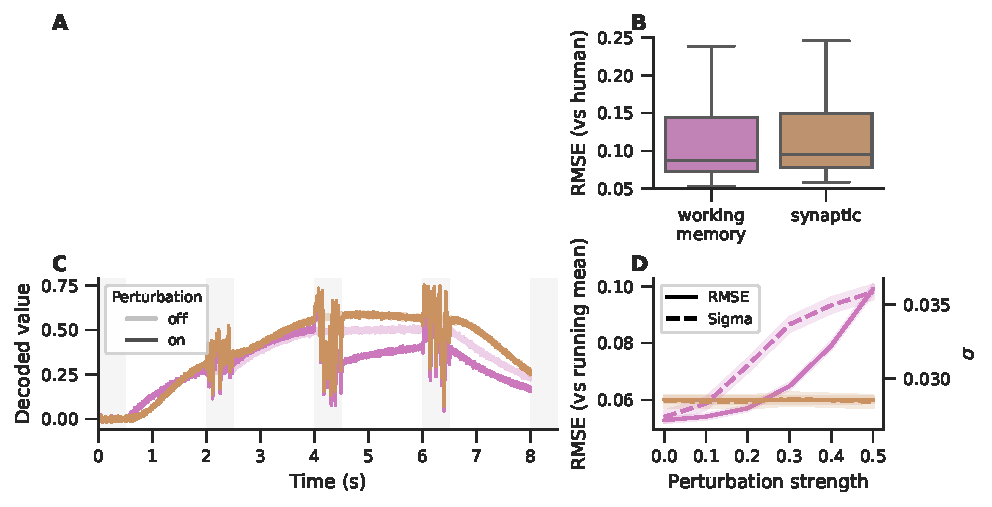
\includegraphics[width=1.0\textwidth]{figures/synaptic_main.pdf}
	\caption{\textbf{A biologically distinct synaptic-plasticity mechanism also fits behavior but predicts different responses to perturbation.} (\textbf{A}) An alternative SNN implements DPE using synaptic plasticity (rather than working memory, WM) via a dopamine-like error-driven learning rule that stores the value estimate in the weights of plastic synapses. (\textbf{B}) On the Continuous Integration task, this synaptic model captures individual human behavior nearly as well as the WM model. (\textbf{C}) Both models' decoding accuracy drops when a simulated perturbation is applied during the intertrial interval (e.g. a distractor task or transcranial stimulation), but only the WM model's disruption persists once the interval ends. (\textbf{D}) Across a range of perturbation strengths, the WM model's error (RMSE vs.\ running mean) and response variability ($\sigma$) both grow with the magnitude of disruption, while the synaptic model is largely unaffected, confirming that only the recurrent, persistent-activity-based mechanism is vulnerable to this kind of transient disruption. This asymmetry reflects each mechanism's dependence on ongoing activity: the WM model needs continuous recurrent feedback to hold its estimate, which is disrupted directly by the perturbation; whereas the synaptic model only changes its stored value in response to a sustained, non-zero-mean error signal, which unstructured noise does not produce. See Discussion for how this dissociation could be tested empirically.}
	\label{fig:synaptic_main}
\end{figure}


%%%%%%%%%%%%%%%% REFERENCES %%%%%%%%%%%%%%%
% Science Advances: <=80 references for a Research Article, ONE combined
% numbered list covering both main text and Supplementary Materials -- no
% separate reference list in the supplement
% (science.org/content/page/science-advances-information-authors).

\clearpage

\bibliography{bibliography}
\bibliographystyle{sciencemag}


%%%%%%%%%%%%%%%% ACKNOWLEDGEMENTS %%%%%%%%%%%%%%%

\section*{Acknowledgments}
\paragraph*{Funding:}
This work was supported by NSF CRCNS grant (BCS2423824) to A.S. We also thank Arthur Prat-Carrabin, Yaomin Jiang, and Ian Krajbich for sharing their empirical data or making them available online.
\paragraph*{Author contributions:}
P.D. and A.S. designed and performed the research; P.D. and A.S. conducted the analyses; A.S. developed the theoretical framework; P.D. built the models, ran simulations, and made the figures; P.D. and A.S. wrote the paper.
\paragraph*{Competing interests:}
There are no competing interests to declare.
\paragraph*{Data, code and materials availability:}
Simulation and analysis code is available on GitHub: \url{https://github.com/psipeter/evidence_integration}.

%%%%%%%%%%%%%%%% SUPPLEMENT LIST %%%%%%%%%%%%%%%
% Add a Tables line here if/when any supplementary tables are added.

%%%%%%%%%%%%%%%% END OF MAIN TEXT %%%%%%%%%%%%%%%

\newpage

%%%%%%%%%%%%%%%% START OF SUPPLEMENT %%%%%%%%%%%%%%%

\renewcommand{\thefigure}{S\arabic{figure}}
\renewcommand{\thetable}{S\arabic{table}}
\renewcommand{\theequation}{S\arabic{equation}}
\renewcommand{\thepage}{S\arabic{page}}
\setcounter{figure}{0}
\setcounter{table}{0}
\setcounter{equation}{0}
\setcounter{page}{1}

\begin{center}
\section*{Supplementary Materials for\\ \scititle}

Peter Duggins$^\ast$,
Alireza Soltani\\
\small$^\ast$Corresponding author. Email: psipeter@gmail.com
\end{center}

\subsubsection*{This PDF file includes:}
Supplementary Text\\
Figures S1 to S3

\newpage

%%%%%%%%%%%%%%%% SUPPLEMENTARY TEXT %%%%%%%%%%%%%%%
% Supplementary Text may only support/elaborate on claims
% already made in the main text, not introduce new ones
% (science.org/content/page/science-advances-information-authors).

\subsection*{Supplementary Text}

\begin{figure} % Do NOT use \begin{figure*} -- single-column template
	\centering
	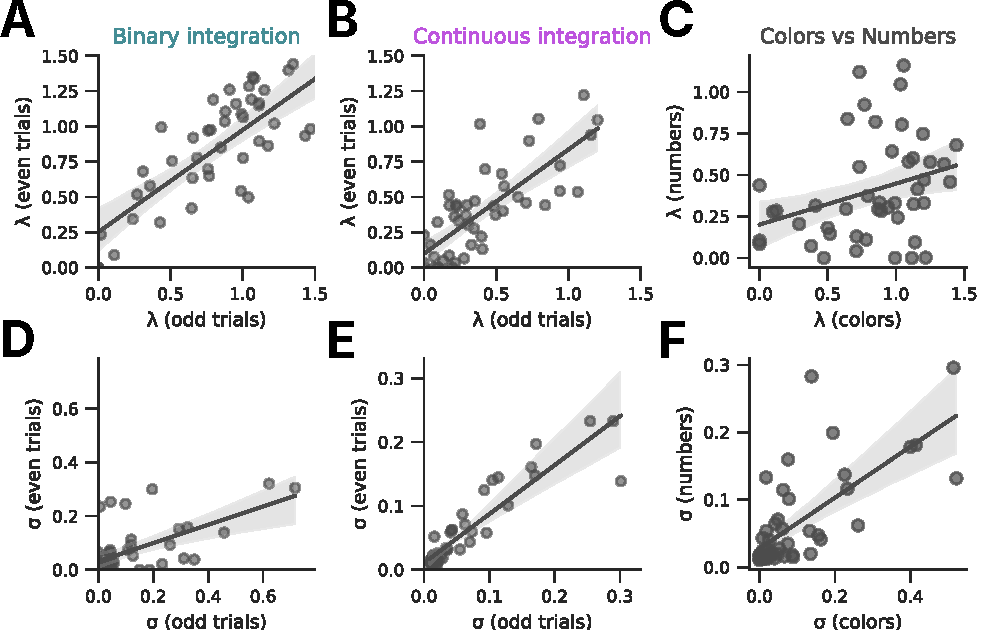
\includegraphics[width=1.0\textwidth]{figures/lambda_sigma_reliability.pdf}
	\caption{\textbf{Participants have consistent response change decay $\lambda$ and response noise $\sigma$ within and across tasks.} (\textbf{A}, \textbf{B}) Split-half (odd/even trial) reliability of fitted $\lambda$ for Binary Integration and Continuous Integration. (\textbf{C}) Across-task consistency of fitted $\lambda$, Binary Integration vs.\ Continuous Integration. (\textbf{D}--\textbf{F}) As in (A--C), for response noise $\sigma$ instead of $\lambda$.}
	\label{fig:lambda_sigma_reliability}
\end{figure}

\subsubsection*{A decoder-free corroboration of the neurons-vs-SNR result}
STUB: add a new supplementary figure showing split-half reliability of
the raw error-population spike counts (\texttt{split\_half\_r\_mean},
already collected in the \texttt{n\_neurons\_snr} grid alongside the
data Fig.~\ref{fig:neural_main}G--I plots, but not yet turned into its
own figure -- see \texttt{scripts/make\_figures.py}'s
\texttt{\_plot\_n\_neurons\_snr\_pair} docstring for the original TODO)
vs.\ n\_neurons. Verified this session: split-half $r$ rises
monotonically with n\_neurons (0.76, 0.85, 0.89, 0.91, 0.93 at
n\_neurons=50, 100, 150, 200, 250) -- this is a fully decoder-free,
purely-neural reliability measure (no decoded PE/value signal
involved), so it corroborates Fig.~\ref{fig:neural_main}G--I's own
PE-noise-vs-n\_neurons finding from a completely independent angle.
Reference this figure from the main text once it exists. TODO: when
drafting this section, discuss the two reliability/noise metrics
together explicitly -- decoded PE noise (coefficient of variation \%,
Fig.~\ref{fig:neural_main}H--I) depends on the value/PE decoders and is
the one reported in the main text, while this figure's split-half
spike-count $r$ is decoder-free -- state plainly that they measure the
same underlying phenomenon (more neurons $\rightarrow$ less spiking
noise $\rightarrow$ more reliable signals) from two independent angles,
one downstream of decoding and one upstream of it.

\begin{figure} % Do NOT use \begin{figure*} -- single-column template
	\centering
	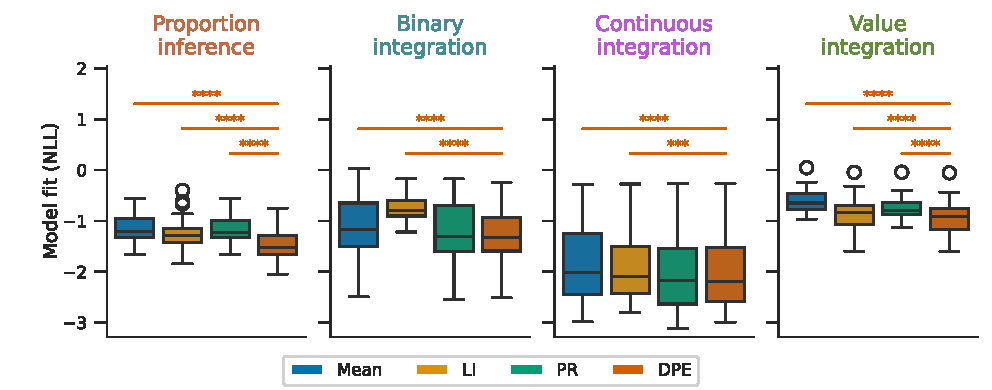
\includegraphics[width=1.0\textwidth]{figures/model_performance_nll.pdf}
	\caption{\textbf{Model performance rankings are consistent under a second fit metric, negative log-likelihood.} As Fig.~\ref{fig:model_performance}, but fit via negative log-likelihood (NLL) instead of RMSE, using each model's own response-noise variant (Mean, LeakyIntegrator (LI), PrimacyRecency (PR), DPE) so that a likelihood is well-defined (stars: paired Wilcoxon vs.\ DPE). (\textbf{A}) Proportion Inference, (\textbf{B}) Binary Integration, (\textbf{C}) Continuous Integration, (\textbf{D}) Value Integration. Rankings match Fig.~\ref{fig:model_performance}'s own RMSE-based comparison: DPE outperforms Mean/LI/PR on Proportion Inference and Value Integration, ties PR on Binary Integration, and loses to PR on Continuous Integration.}
	\label{fig:model_performance_nll}
\end{figure}

\subsubsection*{Model comparison via negative log-likelihood}
STUB: replicate Fig.~\ref{fig:model_performance}'s RMSE-based model comparison using negative log-likelihood (data/runs/nll/, \texttt{\_resp\_noise} model variants) as a second fit metric, across all four tasks (Fig.~\ref{fig:model_performance_nll}). State that the ranking is consistent with the RMSE-based comparison (DPE beats Mean/LI/PR on Proportion Inference and Value Integration; ties PR on Binary Integration; loses to PR on Continuous Integration).

\subsubsection*{Individual differences in temporal discounting: consistency and model comparison}
STUB: report the per-task distribution of fitted $\lambda$ underlying Fig.~\ref{fig:lambda_main}D--F (medians: Binary Integration 0.89, Continuous Integration 0.33, Value Integration 0.16; fraction of participants with $\lambda\geq1$: 39\%, 7\%, 0\% respectively -- Binary Integration is the task with substantial primacy/near-optimal representation). Report within-task split-half (odd/even trial) reliability of fitted $\lambda$ for all three tasks (\texttt{make\_lambda\_reliability}: Value $r$=0.92, Binary $r$=0.78, Continuous $r$=0.78, all $p<10^{-9}$; Binary/Continuous shown in Fig.~\ref{fig:lambda_sigma_reliability}A--B) and across-task consistency for the Binary/Continuous participants who completed both (\texttt{make\_lambda\_sigma\_crosstask}'s $\lambda$ panel, Fig.~\ref{fig:lambda_sigma_reliability}C: $r$=0.31, $p$=0.037) -- note explicitly that across-task consistency, while real, is substantially weaker than within-task reliability. Also explain, with reference to each model's free-parameter roster (CLAUDE.md's "Active models" table), why Mean (no free parameters) cannot produce any individual differences in decay rate, unlike PR/DPE/SNN.

\begin{figure} % Do NOT use \begin{figure*} -- single-column template
	\centering
	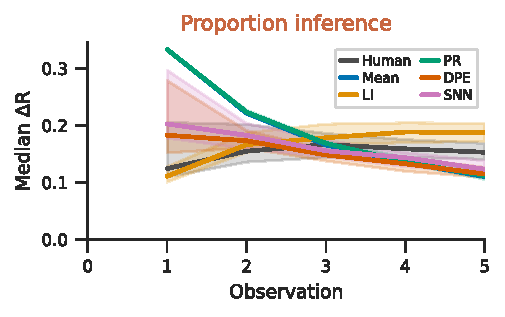
\includegraphics[width=1.0\textwidth]{figures/lambda_balls.pdf}
	\caption{\textbf{Response-change decay is absent in the Proportion Inference task.} As Fig.~\ref{fig:lambda_main}A--C, but for the Proportion Inference task \cite{prat2024imprecise}. Unlike the other three tasks, median $|\Delta R|$ does not decline across the trial's 5 observations. This is likely due to the short sequences used in this task and the response format requested by the task's instructions (see Supplementary Text).}
	\label{fig:lambda_balls}
\end{figure}

\subsubsection*{Response-change decay: the Proportion Inference exception}
STUB: reference Fig.~\ref{fig:lambda_balls}, showing the Proportion Inference (carrabin) task's own response-change-decay panel alongside the same 5 models shown in Fig.~\ref{fig:lambda_main}A--C. State that, unlike the other three tasks, this task's median $|\Delta R|$ does not show a clear decay across the trial's 5 observations, which is also why no per-participant $\lambda$ was ever fit for it (Fig.~\ref{fig:lambda_main}D--F has no corresponding carrabin panel). TODO: the actual explanation for why this task's decay is absent/weaker (e.g. something about its short 5-observation trials or repeated \texttt{qid} sequences vs. the other three tasks' longer, non-repeating ones) still needs to be worked out and written here -- not yet established.

\subsubsection*{Consistency of response noise ($\sigma$) within and across tasks}
STUB: report within-task split-half (odd/even trial) reliability of $\sigma$ for all three tasks (\texttt{make\_sigma\_reliability}: Proportion Inference $r$=0.95, Binary $r$=0.62, Continuous $r$=0.92, all $p<10^{-5}$; Binary/Continuous shown in Fig.~\ref{fig:lambda_sigma_reliability}D--E) and across-task consistency for the Binary/Continuous participants who completed both (\texttt{make\_lambda\_sigma\_crosstask}'s $\sigma$ panel, Fig.~\ref{fig:lambda_sigma_reliability}F: $r$=0.70, $p<10^{-7}$) -- note that $\sigma$'s across-task consistency is considerably stronger than $\lambda$'s own (Fig.~\ref{fig:lambda_sigma_reliability}C: $r$=0.31), worth remarking on directly.

\subsubsection*{State noise vs.\ response noise: growth and autocorrelation of $\sigma$}
STUB: report the actual numbers underlying Fig.~\ref{fig:sigma_main}D--I. Growth (D--F, last-observation/first-observation ratio of normalized $\sigma$): Human grows 1.3--1.9$\times$ across Proportion Inference/Binary/Continuous Integration; all four \texttt{\_resp\_noise} math models are flat (0.93--1.15$\times$, i.e.\ no growth, as expected for i.i.d.\ per-response noise by construction); SNN grows even more than human (2.0--3.2$\times$). Autocorrelation (G--I, lag-1 of the residual from a participant's own typical response): Human is strongly positive (0.40--0.62); all four math models are $\approx$0 (-0.04 to +0.04, pure noise); SNN is strongly positive (0.69--0.76), matching or exceeding human. Discuss \cite{prat2024imprecise}'s own state-vs-response-noise mixture analysis in more detail here, and how it motivated interpreting SNN's spiking noise as a state-noise mechanism.

\end{document}
% End of main.tex